\documentclass[../main.tex]{subfiles}

\begin{document}

\chapter{Об’єктно-орієнтоване проектування ІС}

\section{Архітектурне проектування}

\subsection{Діаграми пакетів}

%TODO explain what each package contain

\begin{figure}[H]
	\centering
	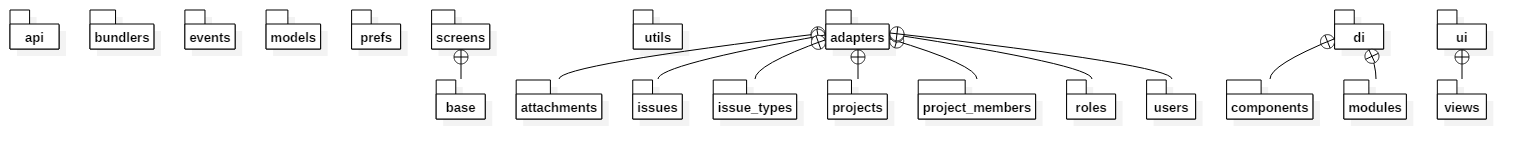
\includegraphics[width=1\textwidth]{3_package_structure_client}
	\caption{Діаграма пакетів Android клієнту}
\end{figure}

\subsection{Діаграми компонентів}

%TODO explain what each class does

\begin{figure}[H]
	\centering
	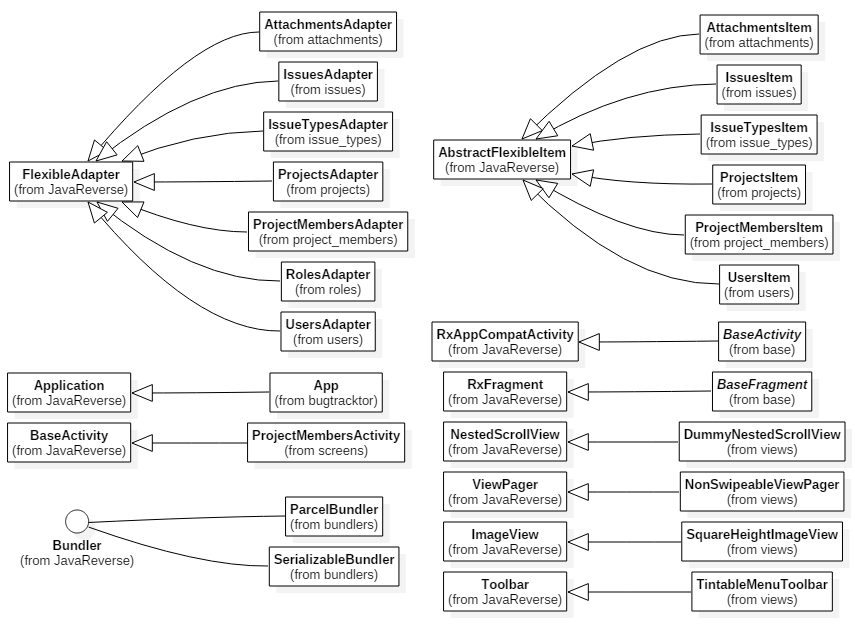
\includegraphics[height=0.9\textheight]{3_hierarchy_client}
	\caption{Діаграма компонентів Android клієнту}
\end{figure}

\section{Детальне проектування}

\begin{figure}[H]
	\centering
	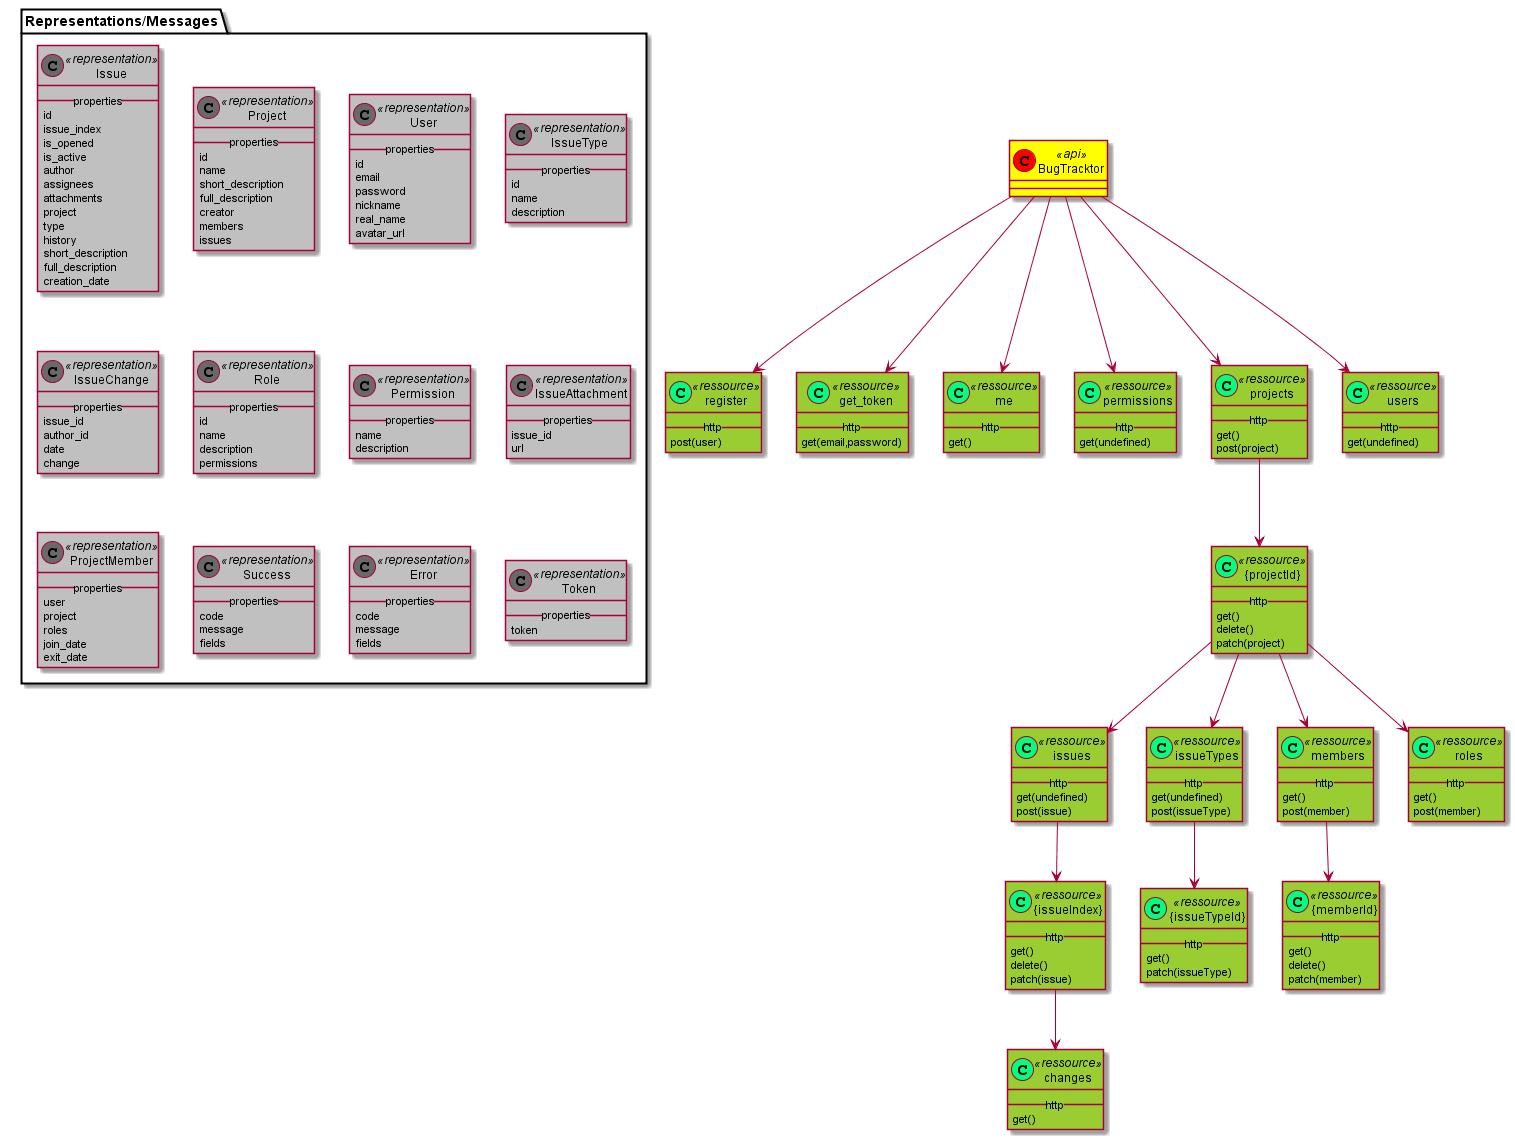
\includegraphics[width=1\textwidth]{3_diagram_rest_api}
	\caption{Діаграма наявних REST ресурсів веб-серверу}
\end{figure}

\begin{figure}[H]
	\centering
	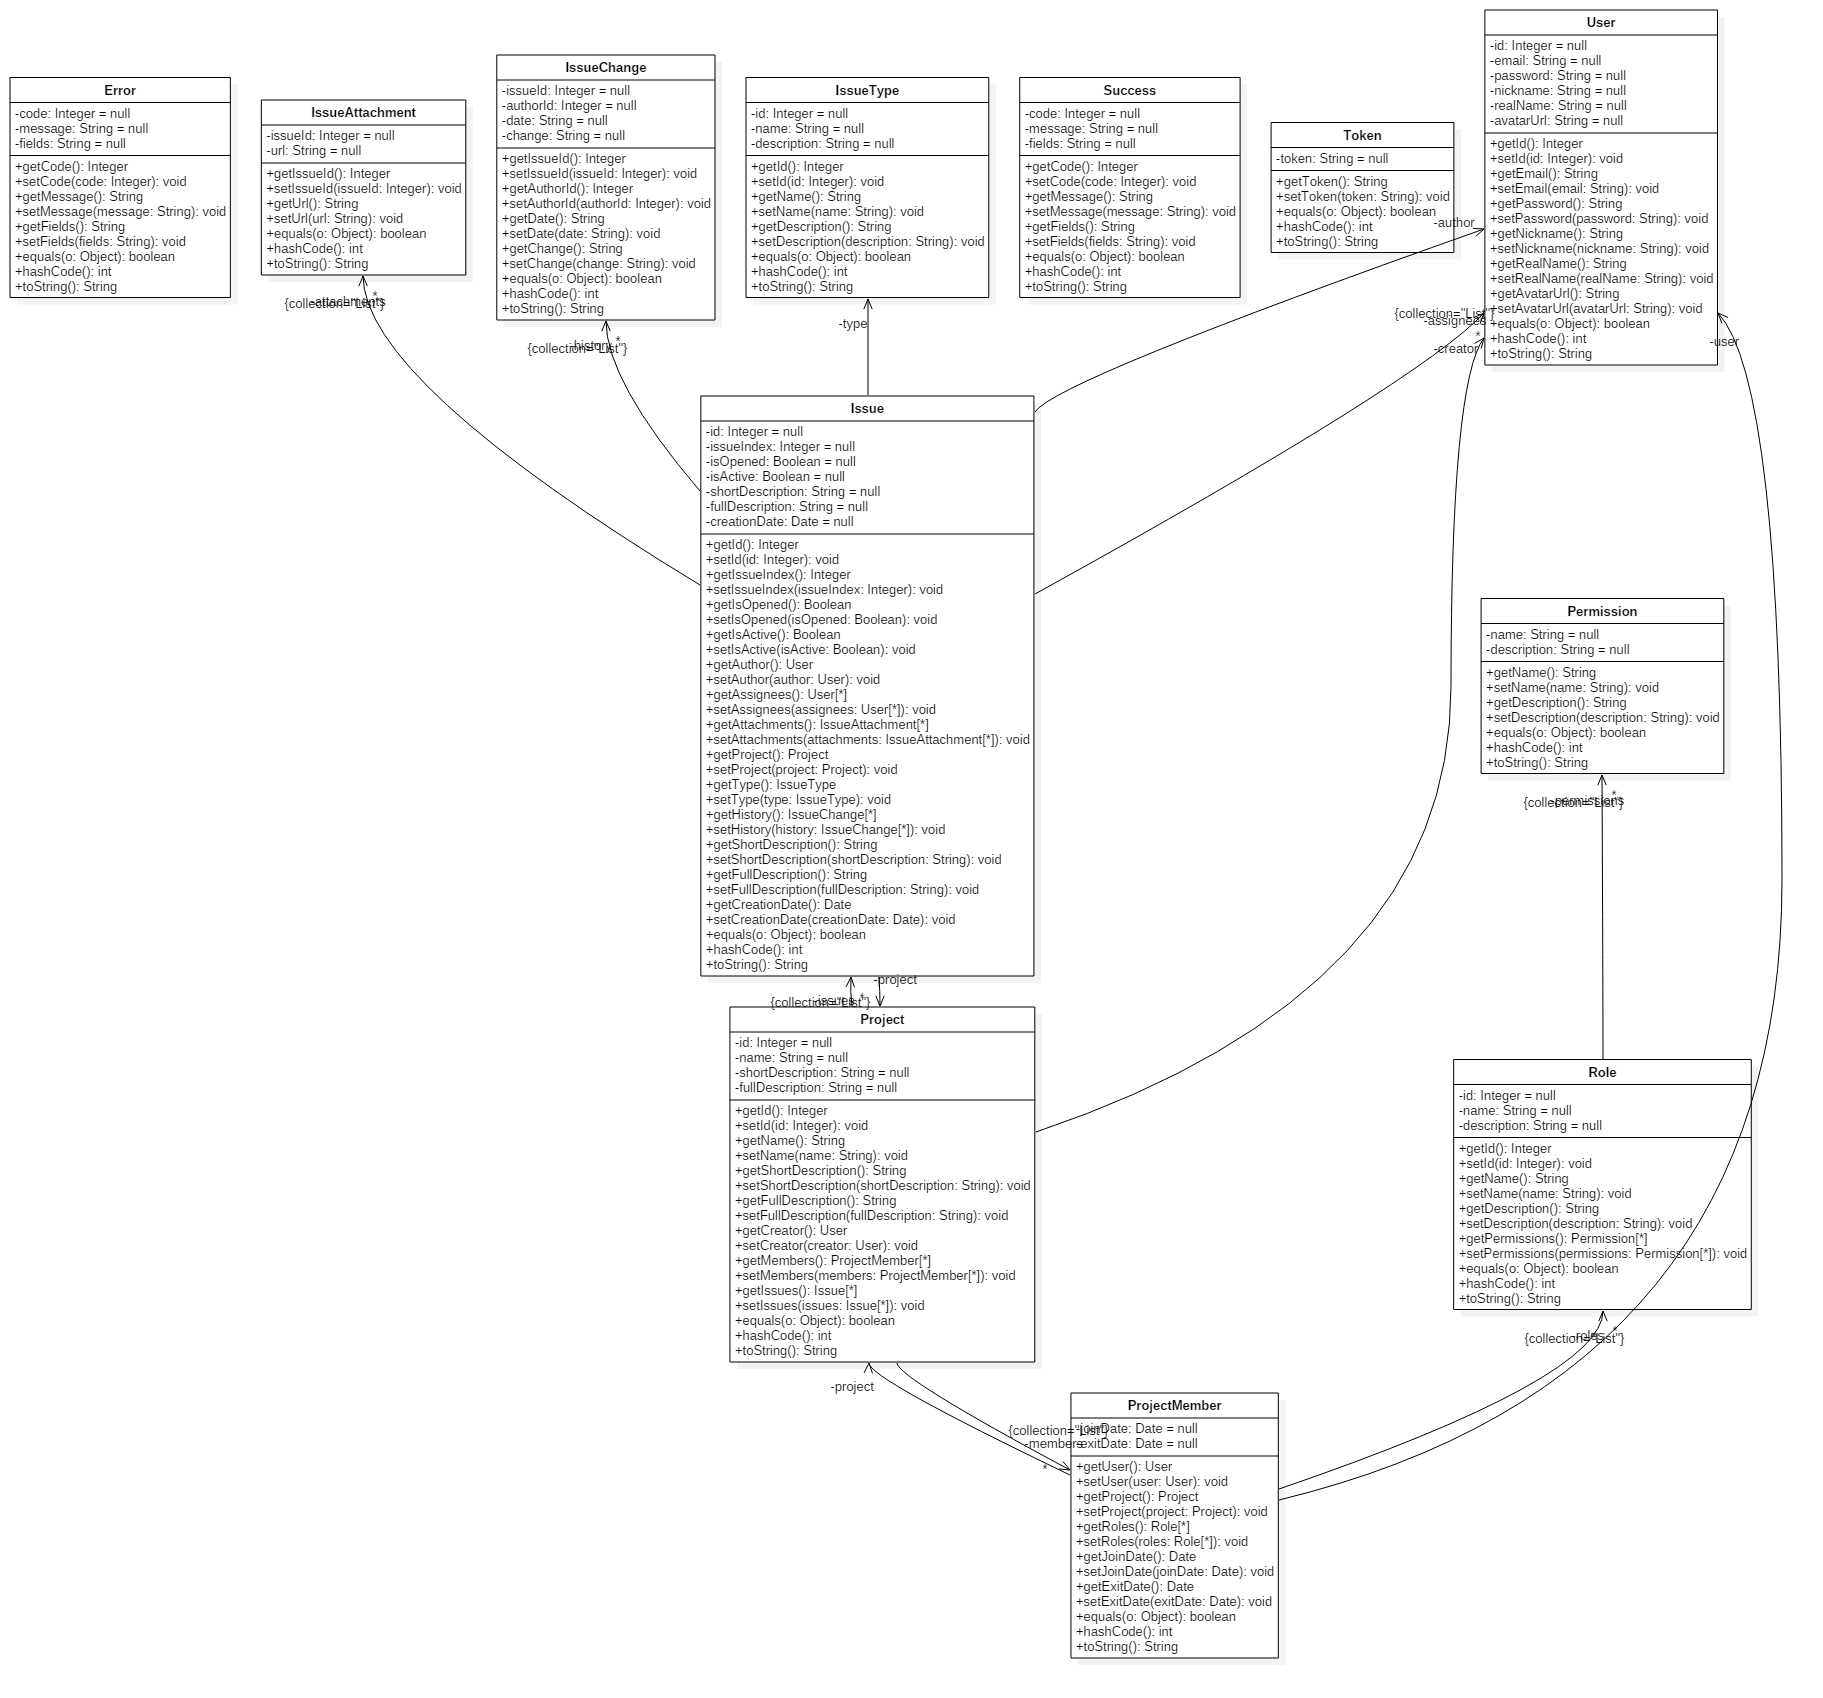
\includegraphics[width=1\textwidth]{3_client_models_diagram}
	\caption{Діаграма моделей даних Android клієнту}
\end{figure}

\begin{figure}[H]
	\centering
	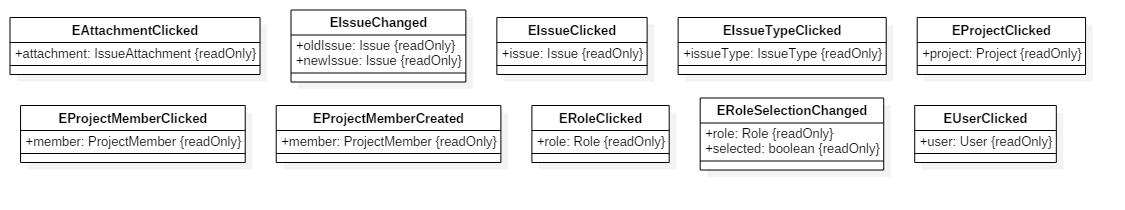
\includegraphics[width=1\textwidth]{3_client_event_classes_diagram}
	\caption{Діаграма класів подій Android клієнту}
\end{figure}

\section{Розгортання програмної системи на апаратних засобах}

\begin{figure}[H]
	\centering
	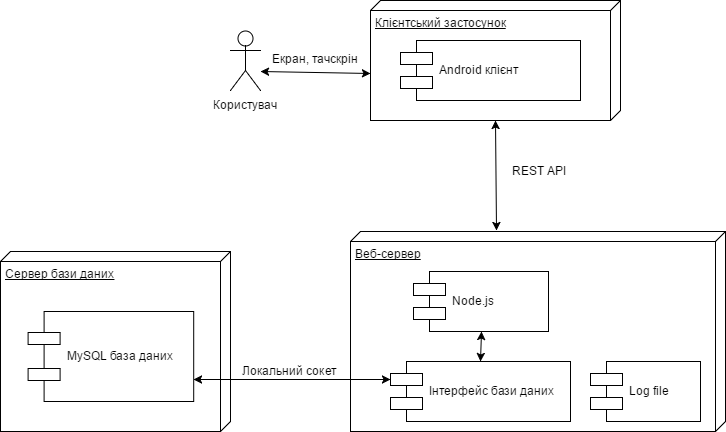
\includegraphics[width=1\textwidth]{3_diagram_deploy}
	\caption{Діаграма розгортання системи}
\end{figure}

\end{document}